\documentclass[12pt]{article}
\usepackage{makeidx}
\usepackage{multirow}
\usepackage{multicol}
\usepackage[dvipsnames,svgnames,table]{xcolor}
\usepackage{graphicx}
\usepackage{epstopdf}
\usepackage{ulem}
\usepackage{hyperref}
\usepackage{amsmath}
\usepackage{amssymb}
\author{Omkar Mohite}
\title{}
\usepackage[paperwidth=595pt,paperheight=841pt,top=72pt,right=72pt,bottom=72pt,left=72pt]{geometry}

\makeatletter
	\newenvironment{indentation}[3]%
	{\par\setlength{\parindent}{#3}
	\setlength{\leftmargin}{#1}       \setlength{\rightmargin}{#2}%
	\advance\linewidth -\leftmargin       \advance\linewidth -\rightmargin%
	\advance\@totalleftmargin\leftmargin  \@setpar{{\@@par}}%
	\parshape 1\@totalleftmargin \linewidth\ignorespaces}{\par}%
\makeatother 

% new LaTeX commands


\begin{document}


\begin{center}
\textbf{{\LARGE Neurosky Mindwave Mobile Headset (EEG sensor)}}
\end{center}

\begin{enumerate}
	\item \textbf{{\large About Neurosky EEG sensor:}}

Measuring EEG activity has traditionally required complex equipment costing thousands of dollars. Now, with our research-grade, embeddable biosensor, NeuroSky has unlocked a new world of affordable solutions for health and wellness, education and entertainment. Precisely accurate, portable, and noise filtering, our EEG biosensors collect electrical signals not actual thoughts to translate brain activity into action.

NeuroSky’s EEG biosensor digitizes and amplifies raw analogue brain signals to deliver concise inputs to games, toys, and devices running health and wellness, educational and research applications. Our brainwave algorithms, developed by NeuroSky neuroscientists and our partner research institutions, have revealed many new ways to interact with our world.


	\item \textbf{{\large EEG Biosensors Features:}}

\begin{enumerate}
	\item \textbf{Basic Features: }
\begin{enumerate}
	\item Direct connect to dry electrode
	\item One EEG channel + Reference + Ground
	\item Extremely low-level signal detection
	\item Advanced filter with high noise immunity
	\item RAW EEG at 512Hz
\end{enumerate}


	\item \textbf{eSense Brainwave Patterns:}


\begin{enumerate}
	\item RAW EEG Signal
	\item Attention
	\item Meditation
	\item Eye Blink
	\item Delta, Theta, low alpha, high alpha, low beta, high beta and gamma waves
\end{enumerate}


	\item \textbf{Dimensions:}


\begin{enumerate}
	\item Size: 2.79cm x 1.52cm x 0.25cm
	\item Weight (Max) 130mg
\end{enumerate}

	\item \textbf{Specifications:}


\begin{enumerate}
	\item 512Hz sampling rate
	\item 3-100Hz frequency range
	\item ESD Ptotection: 4kV Contact Discharge; 8kV Air
	\item Max Power Consumption: 15mA @ 3.3V Operating voltage 2.97 3.63V
\end{enumerate}


	\item \textbf{UART (Serial):}


{\raggedright
1200, 9600, 57600 baud, 8-bits, No parity, 1 stop bit
}
\end{enumerate}
\begin{center}
	\graphicspath{ {images/} }
	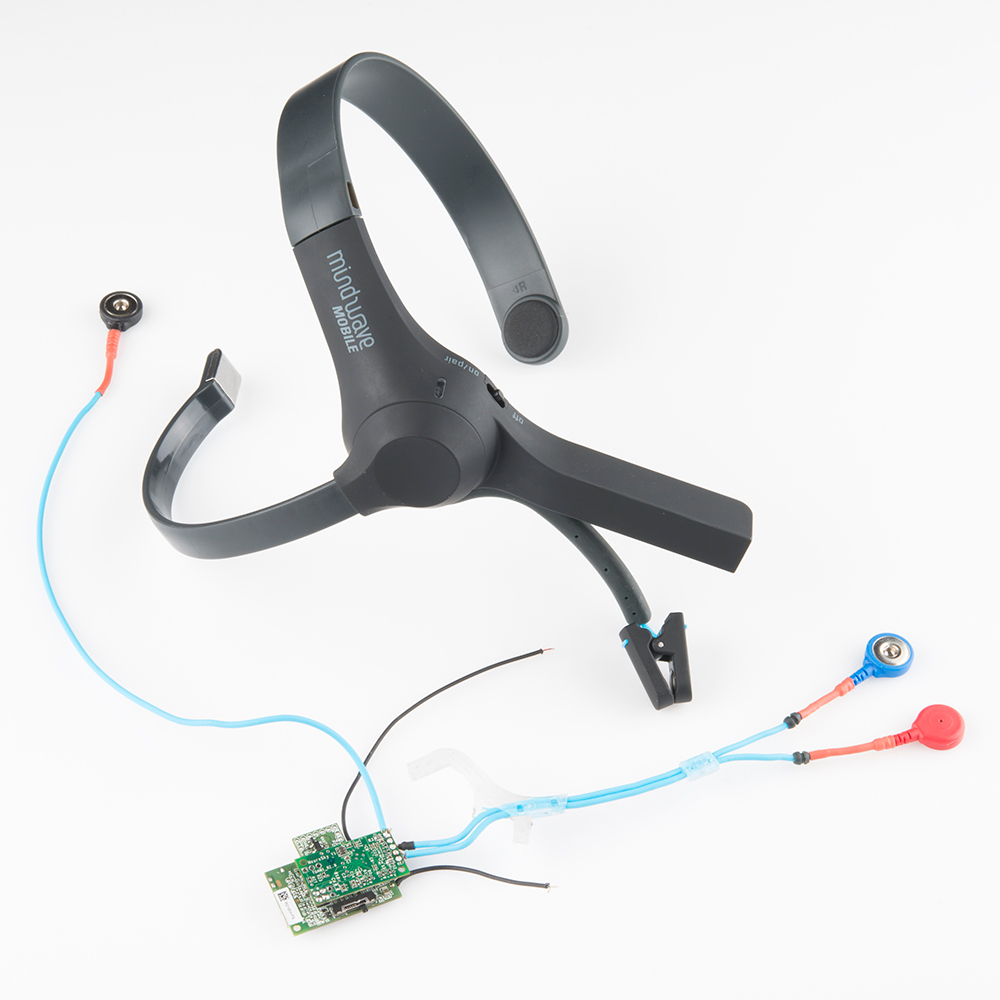
\includegraphics[width=13cm, height=13cm]{EEG_sensor}
\end{center}

	\item \textbf{{\large ThinkGear serial stream guide:}}

\begin{enumerate}
	\item \textbf{Introduction:}



ThinkGear is the technology inside every NeuroSky product or partner product that enables a device to interface with the wearers’ brainwaves. It includes the sensor that touches the forehead, the contact and reference points located on the ear pad, and the onboard chip that processes all of the data and provides this data to software and applications in digital form. Both the raw brainwaves and the eSense Meters (Attention and Meditation) are calculated on the ThinkGear chip.

\begin{enumerate}
	\item 	The ThinkGear Data Values chapter defines the types of Data Values that can be reported by ThinkGear. It is highly recommended that you read this section to familiarize yourself with which kinds of Data Values are (and aren't) available from ThinkGear before continuing to later chapters.
	
	\item The ThinkGear Packets chapter describes the ThinkGear Packet format used to deliver the ThinkGear Data Values.
	\item The ThinkGear Command Bytes chapter is for advanced users and covers how to send Command Bytes to the ThinkGear in order to customize its configuration (change baud rate, enable/disable certain Data Value outputs, etc).
\end{enumerate}


	\item \textbf{{\small ThinkGear Data Values:}}


\begin{enumerate}
	\item \textbf{POOR\_SIGNAL Quality:}


{\raggedright
This unsigned one-byte integer value describes how poor the signal measured by the ThinkGear is. It ranges in value from 0 to 255. Any non-zero value indicates that some sort of noise contamination is detected. The higher the number, the more noise is detected. A value of 200 has a special meaning, specifically that the ThinkGear electrodes aren't contacting a person's skin.
}


	\item \textbf{eSense(tm) meter:}

For all the different types of eSenses (i.e. Attention, Meditation), the meter value is reported on a relative eSense scale of 1 to 100. On this scale, a value between 40 to 60 at any given moment in time is considered “neutral”, and is similar in notion to “baselines” that are established in conventional EEG measurement techniques (though the method for determining a ThinkGear baseline is proprietary and may differ from conventional EEG). A value from 60 to 80 is considered “slightly elevated”, and may be interpreted as levels being possibly higher than normal (levels of Attention or Meditation that may be higher than normal for a given person). Values from 80 to 100 are considered “elevated”, meaning they are strongly indicative of heightened levels of that eSense.

Similarly, on the other end of the scale, a value between 20 and 40 indicates “reduced” levels of the eSense, while a value between 1 and 20 indicates “strongly lowered” levels of the eSense. These levels may indicate states of distraction, agitation, or abnormality, according to the opposite of each eSense. 

An eSense meter value of 0 is a special value indicating the ThinkGear is unable to calculate an eSense level with a reasonable amount of reliability. This may be (and usually is) due to excessive noise as described in the POOR\_SIGNAL Quality section above.
\end{enumerate}
\begin{itemize}
	\item ATTENTION eSense:

This unsigned one-byte value reports the current eSense Attention meter of the user, which indicates the intensity of a user's level of mental “focus” or “attention”, such as that which occurs during intense concentration and directed (but stable) mental activity. Its value ranges from 0 to 100. Distractions, wandering thoughts, lack of focus, or anxiety may lower the Attention meter levels.


	\item MEDITATION eSense:


This unsigned one-byte value reports the current eSense Meditation meter of the user, which indicates the level of a user's mental “calmness” or “relaxation”. Its value ranges from 0 to 100. Note that Meditation is a measure of a person's mental levels, not physical levels.


	\item RAW Wave Value (16-bit):


{\small This Data Value consists of two bytes, and represents a single raw wave sample. Its value is a signed 16-bit integer that ranges from 
	-32768 to 32767.}


	\item  Eye-Blink Strength:

{\small This data value is still unavailable.\\}

\end{itemize}

	\item \textbf{ThinkGear Packets:}
\end{enumerate}

ThinkGear components deliver their digital data as an asynchronous serial stream of bytes. The serial stream must be parsed and interpreted as ThinkGear Packets:

\begin{itemize}
	\item Packet Header
	\item Packet Payload
	\item Payload Checksum
\end{itemize}

\begin{enumerate}
	\item \textbf{Packet Structure}


{\raggedright
{\small [SYNC] [SYNC] [PLENGTH]     [PAYLOAD...]     [CHKSUM]}
}

{\raggedright
{\small \_\_\_\_\_\_\_\_\_\_\_\_\_\_\_\_\_\_\_\_\_\_\_\_\_\_\_\_\_\_\_\_\_\_\_\_ \_\_\_\_\_\_\_\_\_\_\_\_\_\_\_\_\_\_ \_\_\_\_\_\_\_\_\_\_\_\_\_\_\_\_\_\_\_\_}
}

{\raggedright
{\small
\textasciicircum{}\textasciicircum{}\textasciicircum{}\textasciicircum{}\textasciicircum{}\textasciicircum{}\textasciicircum{}\textasciicircum{}(Header)\textasciicircum{}\textasciicircum{}\textasciicircum{}\textasciicircum{}\textasciicircum{}\textasciicircum{}\textasciicircum{}
      \textasciicircum{}\textasciicircum{}
(Payload)\textasciicircum{}\textasciicircum{}    
\textasciicircum{}(Checksum)\textasciicircum{}}
}


	\item \textbf{Packet Header}


The two [SYNC] bytes are used to signal the beginning of a new arriving Packet and are bytes with the value 0xAA (decimal 170). Synchronization is two bytes long, instead of only one, to reduce the chance that [SYNC] (0xAA) bytes occurring within the Packet could be mistaken for the beginning of a Packet.

The [PLENGTH] byte indicates the length, in bytes, of the Packet's Data Payload [PAYLOAD] section, and may be any value from 0 up to 169. Any higher value indicates an error (PLENGTH TOO LARGE). Be sure to note that [PLENGTH] is the length of the Packet's Data Payload, NOT of the entire Packet. The Packet's complete length will always be [PayloadLength] + 4.


	\item \textbf{Data Payload }


The Data Payload of a Packet is simply a series of bytes. The number of Data Payload bytes in the Packet is given by the [PLENGTH] byte from the Packet Header.


	\item \textbf{Payload Checksum}


The [CHKSUM] Byte must be used to verify the integrity of the Packet's Data Payload. The Payload's Checksum is defined as:

\begin{itemize}
	\item 	summing all the bytes of the Packet's Data Payload
	\item 	taking the lowest 8 bits of the sum
	\item   performing the bit inverse (one's compliment inverse) on those lowest 8 bits
\end{itemize}


	\item \textbf{Step-By-Step Guide to Parsing a Packet:}
\end{enumerate}
	\begin{itemize}
	\item 	Keep reading bytes from the stream until a [SYNC] byte (0xAA) is encountered.
	\item Read the next byte and ensure it is also a [SYNC] byte, If not a [SYNC] byte, return to step 1. Otherwise, continue to step 3.
	\item	Read the next byte from the stream as the [PLENGTH]., If [PLENGTH] is 170 ([SYNC]), then repeat step 3., If [PLENGTH] is greater than 170, then return to step 1 (PLENGTH TOO LARGE)., Otherwise, continue to step 4.
	\item Read the next [PLENGTH] bytes of the [PAYLOAD] from the stream, saving them into a storage area (such as an unsigned char payload[256] array). Sum up each byte as it is read by incrementing a checksum accumulator (checksum += byte).
	\item Take the lowest 8 bits of the checksum accumulator and invert them..
	\item Read the next byte from the stream as the[CHKSUM] byte., If the [CHKSUM] does not match your calculated chksum (CHKSUM FAILED). Otherwise, you may now parse the contents of the Payload into DataRows to obtain the Data Values, as described below., In either case, return to step 1.
\end{itemize}


	\item \textbf{	Internal Circuit of Neurosky Mindwave mobile headset:}
\end{enumerate}

The amplitude of rhe EEG is \textasciitilde{} 100 $\mathrm{\mu}$V when measured
on the scalp, and about 1-2 mV when measured on the surface of the brain. The
bandwidth of this signal is from under 1 Hz to about 50 Hz.


The analog brainwaves enter a processing ASIC chip and have digital values that are communicated over Bluetooth. We accessed only the digital data. It is certainly possible to look at the analog brain waves before they enter the processing ASIC, but it would be much more difficult, requiring a schematic and specialized oscilloscope probes.


The Mindwave Mobile was chosen because because it uses Bluetooth, making it easier to interface it with a microcontroller or other hardware. Please note that Neurosky has multiple models of the MindWave.


The ASIC on the Neurosky calculates a value for Attention and Meditation. It also processes five types of brainwaves (more on this shortly) and sends out unitless values for each one. This unit measures eyeblinks too.\\


\textbf{{\large References:}}

\begin{enumerate}
	\item \href{http://neurosky.com/biosensors/eeg-sensor/}{http://neurosky.com/biosensors/eeg-sensor/}
	\item \href{http://neurosky.com/biosensors/eeg-sensor/biosensors/}{http://neurosky.com/biosensors/eeg-sensor/biosensors/}
	\item ThinkGear Serial Stream datasheet (.pdf file present in manuals folder)
\end{enumerate}


\end{document}